\documentclass[a4paper,12pt]{refrep}
\title{Developer Manual}

% Set the page title
\newcommand{\mycontent}[0]{
\begin{tabular}{l}
\hspace*{-4cm} \em XCSoar Developer Manual \vspace*{2pt}
\end{tabular}}

\usepackage{xcolor}

\usepackage{booktabs}
\usepackage{longtable}
\usepackage{rotating}
\usepackage{multicol}
\usepackage{multirow}
\usepackage[disable]{todonotes}
\usepackage[colorlinks=true]{hyperref}
\usepackage{gensymb}
\usepackage{makeidx}\makeindex
\makeatletter
\usepackage{fancyhdr}
\pagestyle{fancy}
\maxipagerulefalse
%
% Include XCSoar header and footer settings and used buttons 
\usepackage{calc}
\usepackage{fancyhdr}

\newcommand{\xcsoarheader}[1]{
\pagestyle{fancy}

% Add XCSoar User Manual title to the header
\fancyhead[L]{
\begin{tabular}{l}
\hspace*{-6cm} \em #1 \vspace*{2pt}
\end{tabular}
}

% Add page number to the footer (centered)
\fancyfoot{}
\fancyfoot[R]{\thepage}
}

% No line between content and header
\renewcommand{\headrulewidth}{0pt}

\fancypagestyle{plain}{
  % Clear fancy header and footer
  \fancyhf{}

  % Add page number to the footer (centered)
  \fancyfoot[R]{\thepage}

  % No line between content and header
  \renewcommand{\headrulewidth}{0pt}
}

\definecolor{buttongray}{rgb}{0.831,0.816,0.784}
\newcommand{\blink}[0]{$\triangleright$}
\newcommand{\bmenu}[1]{
	\fcolorbox {black}{buttongray}{{\sf{#1}}}
}
\newcommand{\bmenut}[2]{
	\fcolorbox {black}{buttongray}{
    \makebox[1.4cm][c]{
    	\begin{tabular}{c}
    	{\footnotesize\sf{#1}}\\
    	{\footnotesize\sf{#2}}
    	\end{tabular}
    }
  }
}
\newcommand{\bmenuth}[3]{
	\fcolorbox {black}{buttongray}{
    \makebox[1.4cm][c]{
    	\begin{tabular}{c}
    	{\footnotesize\sf{#1}}\\
    	{\footnotesize\sf{#2}}\\
    	{\footnotesize\sf{#3}}
    	\end{tabular}
    }
  }
}
\newcommand{\bmenus}[1]{
	\fcolorbox {black}{buttongray}{
    \makebox[1.4cm][c]{
      \begin{tabular}{c}
        {\footnotesize\sf{#1}}\\
    	  \\
      \end{tabular}
	  }
	}
}
\newcommand{\button}[1]{
	\fcolorbox {black}{buttongray}{{\sf #1}}
}

\newcommand{\infobox}[1]{
	\fcolorbox {black}{white}{\makebox[1.7cm][c]{\sf #1}}
}


\newenvironment{jspecs}{
\itemsep=2pt\topsep=3pt\partopsep=3pt\parskip=0pt
\begin{description}
\itemsep=2pt\topsep=3pt\partopsep=3pt\parskip=0pt
}
{\end{description}}

\newcommand{\jindent}[2]{
  \noindent\makebox[0pt][r]{{#1}\hspace*{\marginparsep}}
  \parbox[t]{0.95\linewidth}{#2}\par
}

%
\widowpenalty=1000
\clubpenalty=1000
%
%  XCSoar - Website Einfügen
\newcommand{\xcsoarwebsite}[1]{\url{http://www.xcsoar.org#1}}
%
% Define command to insert tip image
\newcommand{\tip}[0]{\marginlabel{\parbox{1.1cm}{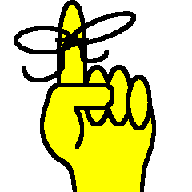
\includegraphics[width=0.7cm]{figures/reminder.pdf}}}}

% Define command to insert gesture image
\newcommand{\gesture}[1]{\marginlabel{{\it#1{\phantom{aa}}}\parbox{1.1cm}{\hspace{-3mm}
\includegraphics[width=0.8cm]{figures/gesture.pdf}}}}
%
% Define command to insert warning image
\newcommand{\warning}[0]{\marginlabel{\parbox{1.3cm}{
\includegraphics[width=0.9cm]{figures/warning.pdf}}}}
%
% Define command to insert Achtung image
\newcommand{\achtung}[0]{\marginlabel{\parbox{1.3cm}{
\includegraphics[width=2.5em]{figures/warning.pdf}}}}
%
% Define command to insert a flash image
\newcommand{\blitz}[0]{\marginlabel{\parbox{1.3cm}{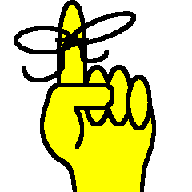
\includegraphics[height=2.0em]{figures/reminder.pdf}}}}
%
% Define command to insert a stop
\newcommand{\halt}[0]{\marginlabel{\parbox{1.3cm}{
\includegraphics[height=2.0em]{figures/warning.pdf}}}}
%
% Define command to reference a configuration item
\newcommand{\config}[1]{\marginlabel{\ref{conf:#1}\parbox{1.3cm}{
\includegraphics[width=0.8cm]{figures/config.pdf}}}}
%
% Potentially overdue ``InfoBox'' style macro but sometimes used... so ..let it be alive ..
\newcommand{\InfoBox}[0]{{InfoBox}}
%
% Define command to put a menu label on the margin
\newcommand{\menulabel}[1]{\marginpar{\parbox{5.0cm}{\raggedright #1}}}
%
% Define command to draw a sketch on the margin
\newcommand{\sketch}[1]{\marginpar{\parbox{4.750cm}{\includegraphics[angle=0,width=0.9\linewidth,keepaspectratio='true']{#1}}}}
%
% Define command to draw a small sketch on the margin
\newcommand{\smallsketch}[1]{\marginpar{\includegraphics[angle=0,keepaspectratio='true']{#1}}}
%
% Enumerated todo's for the todonotes package
\newcounter{todocounter}
\newcommand{\todonum}[2][]{\stepcounter{todocounter}\todo[#1]{\thetodocounter: #2}}
%
% dies nette Makro bringt mir die aktuelle Version der bearbeiteten XCSoar-Verrion aufs Papier 
\newcommand{\version}{\begingroup\catcode`\_=\active\input{VERSION.txt}\endgroup}
%
%Anführungszeichen per Tastatur einfach so eingeben -> "
\shorthandoff{"}%

\def\maketitle{%
  \null
  \thispagestyle{empty}%
  \begin{maxipage}
    \begin{center}
    
\includegraphics[angle=0,width=\textwidth,keepaspectratio='true']{xcsoar-title.png}
    \end{center}
    \begin{center}
      \normalfont\huge\textsf{Glide~Computer and Navigation~System}\par
    \end{center}
    \vskip 1cm
    \begin{center}
      \normalfont\huge\textsf{\@title}\par
    \end{center}
    \vskip 1cm
  \end{maxipage}

  \vfill

  \begin{flushright}
    \large \strut {
      \sf
      \begin{tabular}{r}
      Manual version 1.6 \\
      \today \\
      For XCSoar version 6.0 \\
      \xcsoarwebsite \\
      \end{tabular} 
    } 
    \par
  \end{flushright}
  \par
  \vfil
  \vfil
  \null
  \cleardoublepage
}

\begin{document}
\maketitle

\begingroup
\setlength{\parskip}{0.1\baselineskip}
\tableofcontents
\endgroup

%%%%%%%%%%%%%%%%%%%%%%

\chapter*{Preface}

This manual applies to XCSoar version 6.0.  The authors reserve the
right to update this manual as enhancements are made throughout the
life of this product.

\section*{Warnings and precautions}

\warning IT IS THE USER'S RESPONSIBILITY TO USE THIS SOFTWARE PRUDENTLY. THIS
SOFTWARE IS INTENDED TO BE USED ONLY AS A NAVIGATION AID AND MUST NOT
BE USED FOR ANY PURPOSE REQUIRING PRECISE MEASUREMENT OF DIRECTION,
DISTANCE, LOCATION, OR TOPOGRAPHY. THIS SOFTWARE SHOULD NOT BE USED AS
AN AID TO DETERMINE GROUND PROXIMITY FOR AIRCRAFT NAVIGATION.
THIS SOFTWARE SHOULD NOT BE USED AS A TRAFFIC COLLISION AVOIDANCE SYSTEM.


\section*{Legal notices}

\subsection*{Software license agreement}

This software is released according to the GNU General Public License
Version~2.  See Appendix~\ref{cha:gnu-general-public} for the full
text of the agreement and warranty notice.

\subsection*{Limited liability}

In no event shall XCSoar, or its principals, shareholders, officers,
employees, affiliates, contractors, subsidiaries, or parent
organizations, be liable for any incidental, consequential, or
punitive damages whatsoever relating to the use of the Product.

\subsection*{Disclaimer}

This product, and all accompanying files, data and materials, are
distributed "as is" and with no warranties of any kind, whether
express or implied.  This product is used entirely at the risk of the
user.  Although great care has been taken to eliminate defects during
its development it is not claimed to be fault-free. No claims are made
regarding its correctness, reliability or fitness for any particular
purpose.  The XCSoar project developers and contributors shall not be
liable for errors contained herein or for incidental or consequential
damages, loss of data or personal injury in connection with
furnishing, performance, or use of this material.

%%%%%%%%%%%%%%%%%%%%%%%%%%%%%%%%%%%%%%%%%%%%%%%%%%%%%%%%%%%%%%%%

\chapter{Introduction}\label{cha:introduction}

\chapter{Policy}\label{cha:policy}

\section{Writing Patches}

Submit patches or \texttt{git pull} requests to the developer mailing
list (\texttt{xcsoar-devel@lists.sourceforge.net}).  We provide
accounts on \texttt{git.xcsoar.org} to regular contributors.

A patch should be self-explanatory, it needs a good description.  The
subject line specifies the subsystem/library name and a brief
description of what is changed, followed by an empty line.  Then write
a longer description if needed, and explain why this change is needed.

Each patch must compile and must not introduce a regression (as far as
we know at the time).

Each patch must be self-contained and should only change one thing.
Split larger patches into smaller pieces.  Don't refactor and
add/modify/remove features in the same patch.

Don't rewrite code unless you need to.  Migrate incrementally to a new
concept.  Keep patches small and easy to understand.

\section{Code Style}

79 columns, reasonable exceptions allowed.  Indent 2 spaces, no tabs.

\emph{Comments:} write enough code comments (in English).  All
workarounds must be documented.  Everybody must be able to understand
your code, even when you're gone.

\emph{API documentation:} non-trivial functions should be documented
in a doxygen comment.

\emph{Names:} class/function names in \texttt{CamelCase} (not
\texttt{camelCase}); attributes/variables lower case, separated with
underscore (e.g. \texttt{foo\_bar}); constants (including
\texttt{enum} values) all upper case (e.g. \texttt{FOO\_BAR}).

\emph{Files:} \texttt{*.cpp} and \texttt{*.hpp} for C++.  Files should
be named after the main class which is provided.  Each class should
have a separate source file and a separate header.  UNIX text format.

Be \texttt{const}-correct.

Compile with \texttt{WERROR=y} and fix all warnings.

Don't write large functions.  Split them up when they become too
large.

Avoid dynamic allocation.

Asterisks belong to the variable name, not to the type name.  Consider
``\texttt{Foo* a, b}''.  ``\texttt{Foo *a, b}'' or ``\texttt{Foo *a,
  *b}'' is easier to understand.

Some sample code to demonstrate our code style:

\begin{verbatim}
struct TheStruct {
  unsigned an_attribute;

  void TheMethod();
};

static bool
FooBar(int a_parameter, unsigned another_parameter,
       const TheStruct *next_row)
{
  switch (a_parameter) {
  case 0:
    break;
  }

  if (a_parameter == 2 && another_parameter == 3 &&
      next_row != NULL)
    return true;

  return a_parameter == 42;
}
\end{verbatim}

\section{C++}

Don't use RTTI and exceptions.

Avoid expensive and bloated STL containers if there are cheaper
solutions (e.g. \texttt{StaticArray}, \texttt{StaticString} if the
maximum size is predictable).

Avoid template hell.  Keep templates readable.  Keep in mind that
excessive template use may bloat the binary.

\chapter{Topology and Terrain}\label{cha:topology}
\section{Topology layer description file}
Each line of the topology layer description file (topology.tpl) contains
a comma seperated list (CSV) of information needed for rendering of an
individual topology layer. Lines starting with '*' are ignored.
\begin{table}[ht]
\centering
\sffamily
\begin{tabular}{@{}lll@{}}
\toprule
\addlinespace
Column name&Data type&Valid range\\
%\midrule
\cmidrule(r){1-1}\cmidrule(lr){2-2}\cmidrule(l){3-3}
filename&string&\\
range&double&-\\
icon&-&-\\
label index&-&-\\
color (red component)&int&0-255\\
color (green component)&int&0-255\\
color (blue component)&int&0-255\\
pen width&int&0-31\\
label range&double&-\\
important label range&double&-\\
%\addlinespace
\bottomrule
\end{tabular}
\caption{Topology file format}
\label{tab:topology-file-format}
\end{table}

\begin{description}
\item[filename] The filename of the topology layer within the container file.
\item[range] A threshold zoom level. All layer elements will not be drawn
below this threshold.
\item[pen width] Lines containded within this layer are drawn with pen width.
\item[label range] A threshold zoom level. Labels contained in the layer file
will not be rendered below this threshold.
will not be drawn.
\item[important label range] A threshold zoom level. Labels contained
in the layer file will be rendered in standard style below this threshold.
\end{description}

\appendix

\chapter{GNU General Public License}\label{cha:gnu-general-public}


Ceci est une traduction non officielle de la licence publique générale GNU (GNU GPL) en français (\url{http://www.fsffrance.org/gpl/gpl-fr.fr.html}). Elle n'a pas été publiée par la Free Software Foundation et n'établit pas juridiquement les termes de distribution des logiciels qui utilisent la GNU GPL – seul le texte anglais original de la GNU GPL le fait. Cependant, nous espérons que cette traduction aidera les francophones à mieux comprendre la GNU GPL.\\ 
Le texte original en anglais apparaît ensuite.

This is an unofficial translation of the GNU General Public License into French (\url{http://www.fsffrance.org/gpl/gpl-fr.fr.html}). It was not published by the Free Software Foundation, and does not legally state the distribution terms for software that uses the GNU GPL—only the original English text of the GNU GPL does that. However, we hope that this translation will help French speakers understand the GNU GPL better.\\
The original English text is included after.
\newpage

{\small
	
	\begin{center}
	
Licence Publique Générale GNU

	\end{center}

Les licences de la plupart des logiciels sont conçues pour vous enlever toute liberté de les partager et de les modifier.

A contrario, la Licence Publique Générale est destinée à garantir votre liberté de partager et de modifier les logiciels libres, et à assurer que ces logiciels soient libres pour tous leurs utilisateurs.

La présente Licence Publique Générale s'applique à la plupart des logiciels de la Free Software Foundation, ainsi qu'à tout autre programme pour lequel ses auteurs s'engagent à l'utiliser.

(Certains autres logiciels de la Free Software Foundation sont couverts par la GNU Lesser General Public License à la place.)

Vous pouvez aussi l'appliquer aux programmes qui sont les vôtres.

Quand nous parlons de logiciels libres, nous parlons de liberté, non de prix.

Nos licences publiques générales sont conçues pour vous donner l'assurance d'être libres de distribuer des copies des logiciels libres (et de facturer ce service, si vous le souhaitez), de recevoir le code source ou de pouvoir l'obtenir si vous le souhaitez, de pouvoir modifier les logiciels ou en utiliser des éléments dans de nouveaux programmes libres et de savoir que vous pouvez le faire.

Pour protéger vos droits, il nous est nécessaire d'imposer des limitations qui interdisent à quiconque de vous refuser ces droits ou de vous demander d'y renoncer.

Certaines responsabilités vous incombent en raison de ces limitations si vous distribuez des copies de ces logiciels, ou si vous les modifiez.

Par exemple, si vous distribuez des copies d'un tel programme, à titre gratuit ou contre une rémunération, vous devez accorder aux destinataires tous les droits dont vous disposez.

Vous devez vous assurer qu'eux aussi reçoivent ou puissent disposer du code source.

Et vous devez leur montrer les présentes conditions afin qu'ils aient connaissance de leurs droits.

Nous protégeons vos droits en deux étapes : (1) nous sommes titulaires des droits d'auteur du logiciel, et (2) nous vous délivrons cette licence, qui vous donne l'autorisation légale de copier, distribuer et/ou modifier le logiciel.

En outre, pour la protection de chaque auteur ainsi que la nôtre, nous voulons nous assurer que chacun comprenne que ce logiciel libre ne fait l'objet d'aucune garantie.

Si le logiciel est modifié par quelqu'un d'autre puis transmis à des tiers, nous voulons que les destinataires soient mis au courant que ce qu'ils ont reçu n'est pas le logiciel d'origine, de sorte que tout problème introduit par d'autres ne puisse entacher la réputation de l'auteur originel.

En définitive, un programme libre restera à la merci des brevets de logiciels.

Nous souhaitons éviter le risque que les redistributeurs d'un programme libre fassent des demandes individuelles de licence de brevet, ceci ayant pour effet de rendre le programme propriétaire.

Pour éviter cela, nous établissons clairement que toute licence de brevet doit être concédée de façon à ce que l'usage en soit libre pour tous ou bien qu'aucune licence ne soit concédée.

Les termes exacts et les conditions de copie, distribution et modification sont les suivants:
Conditions de copie, distribution et modification de la Licence Publique Générale GNU.

	\begin{enumerate}

\item La présente Licence s'applique à tout programme ou tout autre ouvrage contenant un avis, apposé par le titulaire des droits d'auteur, stipulant qu'il peut être distribué au titre des conditions de la présente Licence Publique Générale.

Ci-après, le "Programme" désigne l'un quelconque de ces programmes ou ouvrages, et un "ouvrage fondé sur le Programme" désigne soit le Programme, soit un ouvrage qui en dérive au titre des lois sur le droit d'auteur : en d'autres termes, un ouvrage contenant le Programme ou une partie de ce dernier, soit à l'identique, soit avec des modifications et/ou traduit dans un autre langage.

(Ci-après, le terme "modification" implique, sans s'y réduire, le terme traduction)

Chaque concessionaire sera désigné par "vous".

Les activités autres que la copie, la distribution et la modification ne sont pas couvertes par la présente Licence ; elles sont hors de son champ d'application.

L'opération consistant à exécuter le Programme n'est soumise à aucune limitation et les sorties du programme ne sont couvertes que si leur contenu constitue un ouvrage fondé sur le Programme (indépendamment du fait qu'il ait été réalisé par l'exécution du Programme).

La validité de ce qui précède dépend de ce que fait le Programme.

\item  Vous pouvez copier et distribuer des copies à l'identique du code source du Programme tel que vous l'avez reçu, sur n'importe quel support, du moment que vous apposiez sur chaque copie, de manière ad hoc et parfaitement visible, l'avis de droit d'auteur adéquat et une exonération de garantie ; que vous gardiez intacts tous les avis faisant référence à la présente Licence et à l'absence de toute garantie ; et que vous fournissiez à tout destinataire du Programme autre que vous-même un exemplaire de la présente Licence en même temps que le Programme.

Vous pouvez faire payer l'acte physique de transmission d'une copie, et vous pouvez, à votre discrétion, proposer une garantie contre rémunération.

\item  Vous pouvez modifier votre copie ou des copies du Programme ou n'importe quelle partie de celui-ci, créant ainsi un ouvrage fondé sur le Programme, et copier et distribuer de telles modifications ou ouvrage selon les termes de l'Article 1 ci-dessus, à condition de vous conformer également à chacune des obligations suivantes :


\begin{enumerate}
\item Vous devez munir les fichiers modifiés d'avis bien visibles stipulants que vous avez modifié ces fichiers, ainsi que la date de chaque modification ;

\item Vous devez prendre les dispositions nécessaires pour que tout ouvrage que vous distribuez ou publiez, et qui, en totalité ou en partie, contient ou est fondé sur le Programme - ou une partie quelconque de ce dernier - soit concédé comme un tout, à titre gratuit, à n'importe quel tiers, au titre des conditions de la présente Licence.

\item Si le programme modifié lit habituellement des instructions de façon interactive lorsqu'on l'exécute, vous devez, quand il commence son exécution pour ladite utilisation interactive de la manière la plus usuelle, faire en sorte qu'il imprime ou affiche une annonce comprenant un avis de droit d'auteur ad hoc, et un avis stipulant qu'il n'y a pas de garantie (ou bien indiquant que c'est vous qui fournissez la garantie), et que les utilisateurs peuvent redistribuer le programme en respectant les présentes obligations, et expliquant à l'utilisateur comment voir une copie de la présente Licence.


\end{enumerate}
(Exception : si le Programme est lui-même interactif mais n'imprime pas habituellement une telle annonce, votre ouvrage fondé sur le Programme n'est pas obligé d'imprimer une annonce).

Ces obligations s'appliquent à l'ouvrage modifié pris comme un tout.

Si des éléments identifiables de cet ouvrage ne sont pas fondés sur le Programme et peuvent raisonnablement être considérés comme des ouvrages indépendants distincts en eux mêmes, alors la présente Licence et ses conditions ne s'appliquent pas à ces éléments lorsque vous les distribuez en tant qu'ouvrages distincts.

Mais lorsque vous distribuez ces mêmes éléments comme partie d'un tout, lequel constitue un ouvrage fondé sur le Programme, la distribution de ce tout doit être soumise aux conditions de la présente Licence, et les autorisations qu'elle octroie aux autres concessionnaires s'étendent à l'ensemble de l'ouvrage et par conséquent à chaque et toute partie indifférement de qui l'a écrite.

Par conséquent, l'objet du présent article n'est pas de revendiquer des droits ou de contester vos droits sur un ouvrage entièrement écrit par vous; son objet est plutôt d'exercer le droit de contrôler la distribution d'ouvrages dérivés ou d'ouvrages collectifs fondés sur le Programme.

De plus, la simple proximité du Programme avec un autre ouvrage qui n'est pas fondé sur le Programme (ou un ouvrage fondé sur le Programme) sur une partition d'un espace de stockage ou un support de distribution ne place pas cet autre ouvrage dans le champ d'application de la présente Licence.

\item  Vous pouvez copier et distribuer le Programme (ou un ouvrage fondé sur lui, selon l'Article 2) sous forme de code objet ou d'exécutable, selon les termes des Articles 1 et 2 ci-dessus, à condition que vous accomplissiez l'un des points suivants :


\begin{enumerate}
\item L'accompagner de l'intégralité du code source correspondant, sous une forme lisible par un ordinateur, lequel doit être distribué au titre des termes des Articles 1 et 2 ci-dessus, sur un support habituellement utilisé pour l'échange de logiciels; ou,

\item L'accompagner d'une proposition écrite, valable pendant au moins trois ans, de fournir à tout tiers, à un tarif qui ne soit pas supérieur à ce que vous coûte l'acte physique de réaliser une distribution source, une copie intégrale du code source correspondant sous une forme lisible par un ordinateur, qui sera distribuée au titre des termes des Articles 1 et 2 ci-dessus, sur un support habituellement utilisé pour l'échange de logiciels; ou,

\item  L'accompagner des informations reçues par vous concernant la proposition de distribution du code source correspondant. (Cette solution n'est autorisée que dans le cas d'une distribution non commerciale et seulement si vous avez reçu le programme sous forme de code objet ou d'exécutable accompagné d'une telle proposition - en conformité avec le sous-Article b ci-dessus.)
\end{enumerate}

Le code source d'un ouvrage désigne la forme favorite pour travailler à des modifications de cet ouvrage. Pour un ouvrage exécutable, le code source intégral désigne la totalité du code source de la totalité des modules qu'il contient, ainsi que les éventuels fichiers de définition des interfaces qui y sont associés, ainsi que les scripts utilisés pour contrôler la compilation et l'installation de l'exécutable. Cependant, par exception spéciale, le code source distribué n'est pas censé inclure quoi que ce soit de normalement distribué (que ce soit sous forme source ou binaire) avec les composants principaux (compilateur, noyau, et autre) du système d'exploitation sur lequel l'exécutable tourne, à moins que ce composant lui-même n'accompagne l'exécutable.

Si distribuer un exécutable ou un code objet consiste à offrir un accès permettant leur copie depuis un endroit particulier, alors l'offre d'un accès équivalent pour copier le code source depuis le même endroit compte comme une distribution du code source - même si les tiers ne sont pas contraints de copier le source en même temps que le code objet.

\item  Vous ne pouvez copier, modifier, concéder en sous-licence, ou distribuer le Programme, sauf tel qu'expressément prévu par la présente Licence. Toute tentative de copier, modifier, concéder en sous-licence, ou distribuer le Programme d'une autre manière est réputée non valable, et met immédiatement fin à vos droits au titre de la présente Licence. Toutefois, les tiers ayant reçu de vous des copies, ou des droits, au titre de la présente Licence ne verront pas leurs autorisations résiliées aussi longtemps que ledits tiers se conforment pleinement à elle.

\item  Vous n'êtes pas obligé d'accepter la présente Licence étant donné que vous ne l'avez pas signée. Cependant, rien d'autre ne vous accorde l'autorisation de modifier ou distribuer le Programme ou les ouvrages fondés sur lui. Ces actions sont interdites par la loi si vous n'acceptez pas la présente Licence. En conséquence, en modifiant ou distribuant le Programme (ou un ouvrage quelconque fondé sur le Programme), vous signifiez votre acceptation de la présente Licence en le faisant, et de toutes ses conditions concernant la copie, la distribution ou la modification du Programme ou d'ouvrages fondés sur lui.

\item  Chaque fois que vous redistribuez le Programme (ou n'importe quel ouvrage fondé sur le Programme), une licence est automatiquement concédée au destinataire par le concédant originel de la licence, l'autorisant à copier, distribuer ou modifier le Programme, sous réserve des présentes conditions. Vous ne pouvez imposer une quelconque limitation supplémentaire à l'exercice des droits octroyés au titre des présentes par le destinataire. Vous n'avez pas la responsabilité d'imposer le respect de la présente Licence à des tiers.

\item  Si, conséquement à une décision de justice ou l'allégation d'une transgression de brevet ou pour toute autre raison (non limitée à un probleme de brevet), des obligations vous sont imposées (que ce soit par jugement, conciliation ou autre) qui contredisent les conditions de la présente Licence, elles ne vous excusent pas des conditions de la présente Licence. Si vous ne pouvez distribuer de manière à satisfaire simultanément vos obligations au titre de la présente Licence et toute autre obligation pertinente, alors il en découle que vous ne pouvez pas du tout distribuer le Programme. Par exemple, si une licence de brevet ne permettait pas une redistribution sans redevance du Programme par tous ceux qui reçoivent une copie directement ou indirectement par votre intermédiaire, alors la seule façon pour vous de satisfaire à la fois à la licence du brevet et à la présente Licence serait de vous abstenir totalement de toute distribution du Programme.

Si une partie quelconque de cet article est tenue pour nulle ou inopposable dans une circonstance particulière quelconque, l'intention est que le reste de l'article s'applique. La totalité de la section s'appliquera dans toutes les autres circonstances.

Cet article n'a pas pour but de vous induire à transgresser un quelconque brevet ou d'autres revendications à un droit de propriété ou à contester la validité de la moindre de ces revendications ; cet article a pour seul objectif de protéger l'intégrité du système de distribution du logiciel libre, qui est mis en oeuvre par la pratique des licenses publiques. De nombreuses personnes ont fait de généreuses contributions au large spectre de logiciels distribués par ce système en se fiant à l'application cohérente de ce système ; il appartient à chaque auteur/donateur de décider si il ou elle veut distribuer du logiciel par l'intermédiaire d'un quelconque autre système et un concessionaire ne peut imposer ce choix.

Cet article a pour but de rendre totalement limpide ce que l'on pense être une conséquence du reste de la présente Licence.

\item  Si la distribution et/ou l'utilisation du Programme est limitée dans certains pays que ce soit par des brevets ou par des interfaces soumises au droit d'auteur, le titulaire originel des droits d'auteur qui décide de couvrir le Programme par la présente Licence peut ajouter une limitation géographique de distribution explicite qui exclue ces pays afin que la distribution soit permise seulement dans ou entre les pays qui ne sont pas ainsi exclus. Dans ce cas, la présente Licence incorpore la limitation comme si elle était écrite dans le corps de la présente Licence.

\item  La Free Software Foundation peut, de temps à autre, publier des versions révisées et/ou nouvelles de la Licence Publique Générale. De telles nouvelles versions seront similaires à la présente version dans l'esprit mais pourront différer dans le détail pour prendre en compte de nouvelles problématiques ou inquiétudes.

Chaque version possède un numéro de version la distinguant. Si le Programme précise le numéro de version de la présente Licence qui s'y applique et "une version ultérieure quelconque", vous avez le choix de suivre les conditions de la présente version ou de toute autre version ultérieure publiée par la Free Software Foundation. Si le Programme ne spécifie aucun numéro de version de la présente Licence, vous pouvez choisir une version quelconque publiée par la Free Software Foundation à quelque moment que ce soit.

\item  Si vous souhaitez incorporer des parties du Programme dans d'autres programmes libres dont les conditions de distribution sont différentes, écrivez à l'auteur pour lui en demander l'autorisation. Pour les logiciels dont la Free Software Foundation est titulaire des droits d'auteur, écrivez à la Free Software Foundation ; nous faisons parfois des exceptions dans ce sens. Notre décision sera guidée par le double objectif de préserver le statut libre de tous les dérivés de nos logiciels libres et de promouvoir le partage et la réutilisation des logiciels en général.
ABSENCE DE GARANTIE

\item  COMME LA LICENCE DU PROGRAMME EST CONCEDEE A TITRE GRATUIT, AUCUNE GARANTIE NE S'APPLIQUE AU PROGRAMME, DANS LES LIMITES AUTORISEES PAR LA LOI APPLICABLE. SAUF MENTION CONTRAIRE ECRITE, LES TITULAIRES DU DROIT D'AUTEUR ET/OU LES AUTRES PARTIES FOURNISSENT LE PROGRAMME "EN L'ETAT", SANS AUCUNE GARANTIE DE QUELQUE NATURE QUE CE SOIT, EXPRESSE OU IMPLICITE, Y COMPRIS, MAIS SANS Y ETRE LIMITE, LES GARANTIES IMPLICITES DE COMMERCIABILITE ET DE LA CONFORMITE A UNE UTILISATION PARTICULIERE. VOUS ASSUMEZ LA TOTALITE DES RISQUES LIES A LA QUALITE ET AUX PERFORMANCES DU PROGRAMME. SI LE PROGRAMME SE REVELAIT DEFECTUEUX, LE COUT DE L'ENTRETIEN, DES REPARATIONS OU DES CORRECTIONS NECESSAIRES VOUS INCOMBENT INTEGRALEMENT.

\item  EN AUCUN CAS, SAUF LORSQUE LA LOI APPLICABLE OU UNE CONVENTION ECRITE L'EXIGE, UN TITULAIRE DE DROIT D'AUTEUR QUEL QU'IL SOIT, OU TOUTE PARTIE QUI POURRAIT MODIFIER ET/OU REDISTRIBUER LE PROGRAMME COMME PERMIS CI-DESSUS, NE POURRAIT ETRE TENU POUR RESPONSABLE A VOTRE EGARD DES DOMMAGES, INCLUANT LES DOMMAGES GENERIQUES, SPECIFIQUES, SECONDAIRES OU CONSECUTIFS, RESULTANT DE L'UTILISATION OU DE L'INCAPACITE D'UTILISER LE PROGRAMME (Y COMPRIS, MAIS SANS Y ETRE LIMITE, LA PERTE DE DONNEES, OU LE FAIT QUE DES DONNEES SOIENT RENDUES IMPRECISES, OU LES PERTES EPROUVEES PAR VOUS OU PAR DES TIERS, OU LE FAIT QUE LE PROGRAMME ECHOUE A INTEROPERER AVEC UN AUTRE PROGRAMME QUEL QU'IL SOIT) MEME SI LE DIT TITULAIRE DU DROIT D'AUTEUR OU LE PARTIE CONCERNEE A ETE AVERTI DE L'EVENTUALITE DE TELS DOMMAGES.

		\end{enumerate}


FIN DES CONDITIONS

\vspace{1cm}
Sur les pages suivantes, la version original en anglais de la General Public License. 
\newpage 

	\begin{center}
		GNU GENERAL PUBLIC LICENSE
		
		Version 2, June 1991
		
		
	\end{center}
	
	Copyright (C) 1989, 1991 Free Software Foundation, Inc.
	
	59 Temple Place, Suite 330, Boston, MA  02111-1307  USA
	
	Everyone is permitted to copy and distribute verbatim copies
	of this license document, but changing it is not allowed.
	
	\begin{center}
		Preamble
	\end{center}
	
	The licenses for most software are designed to take away your
	freedom to share and change it.  By contrast, the GNU General Public
	License is intended to guarantee your freedom to share and change free
	software--to make sure the software is free for all its users.  This
	General Public License applies to most of the Free Software
	Foundation's software and to any other program whose authors commit to
	using it.  (Some other Free Software Foundation software is covered by
	the GNU Library General Public License instead.)  You can apply it to
	your programs, too.
	
	When we speak of free software, we are referring to freedom, not
	price.  Our General Public Licenses are designed to make sure that you
	have the freedom to distribute copies of free software (and charge for
	this service if you wish), that you receive source code or can get it
	if you want it, that you can change the software or use pieces of it
	in new free programs; and that you know you can do these things.
	
	To protect your rights, we need to make restrictions that forbid
	anyone to deny you these rights or to ask you to surrender the rights.
	These restrictions translate to certain responsibilities for you if you
	distribute copies of the software, or if you modify it.
	
	For example, if you distribute copies of such a program, whether
	gratis or for a fee, you must give the recipients all the rights that
	you have.  You must make sure that they, too, receive or can get the
	source code.  And you must show them these terms so they know their
	rights.
	
	We protect your rights with two steps: (1) copyright the software, and
	(2) offer you this license which gives you legal permission to copy,
	distribute and/or modify the software.
	
	Also, for each author's protection and ours, we want to make certain
	that everyone understands that there is no warranty for this free
	software.  If the software is modified by someone else and passed on, we
	want its recipients to know that what they have is not the original, so
	that any problems introduced by others will not reflect on the original
	authors' reputations.
	
	Finally, any free program is threatened constantly by software
	patents.  We wish to avoid the danger that redistributors of a free
	program will individually obtain patent licenses, in effect making the
	program proprietary.  To prevent this, we have made it clear that any
	patent must be licensed for everyone's free use or not licensed at all.
	
	The precise terms and conditions for copying, distribution and
	modification follow.
	
	\begin{center}
		GNU GENERAL PUBLIC LICENSE
		
		TERMS AND CONDITIONS FOR COPYING, DISTRIBUTION AND MODIFICATION
	\end{center}
	
	\begin{enumerate}
		\item This License applies to any program or other work which contains
		a notice placed by the copyright holder saying it may be distributed
		under the terms of this General Public License.  The ``Program'', below,
		refers to any such program or work, and a ``work based on the Program''
		means either the Program or any derivative work under copyright law:
		that is to say, a work containing the Program or a portion of it,
		either verbatim or with modifications and/or translated into another
		language.  (Hereinafter, translation is included without limitation in
		the term ``modification''.)  Each licensee is addressed as ``you''.
		
		Activities other than copying, distribution and modification are not
		covered by this License; they are outside its scope.  The act of
		running the Program is not restricted, and the output from the Program
		is covered only if its contents constitute a work based on the
		Program (independent of having been made by running the Program).
		Whether that is true depends on what the Program does.
		
		\item You may copy and distribute verbatim copies of the Program's
		source code as you receive it, in any medium, provided that you
		conspicuously and appropriately publish on each copy an appropriate
		copyright notice and disclaimer of warranty; keep intact all the
		notices that refer to this License and to the absence of any warranty;
		and give any other recipients of the Program a copy of this License
		along with the Program.
		
		You may charge a fee for the physical act of transferring a copy, and
		you may at your option offer warranty protection in exchange for a fee.
		
		\item You may modify your copy or copies of the Program or any portion
		of it, thus forming a work based on the Program, and copy and
		distribute such modifications or work under the terms of Section 1
		above, provided that you also meet all of these conditions:
		
		\begin{enumerate}
			\item You must cause the modified files to carry prominent notices
			stating that you changed the files and the date of any change.
			
			\item You must cause any work that you distribute or publish, that in
			whole or in part contains or is derived from the Program or any
			part thereof, to be licensed as a whole at no charge to all third
			parties under the terms of this License.
			
			\item If the modified program normally reads commands interactively
			when run, you must cause it, when started running for such
			interactive use in the most ordinary way, to print or display an
			announcement including an appropriate copyright notice and a
			notice that there is no warranty (or else, saying that you provide
			a warranty) and that users may redistribute the program under
			these conditions, and telling the user how to view a copy of this
			License.  (Exception: if the Program itself is interactive but
			does not normally print such an announcement, your work based on
			the Program is not required to print an announcement.)
		\end{enumerate}
		
		These requirements apply to the modified work as a whole.  If
		identifiable sections of that work are not derived from the Program,
		and can be reasonably considered independent and separate works in
		themselves, then this License, and its terms, do not apply to those
		sections when you distribute them as separate works.  But when you
		distribute the same sections as part of a whole which is a work based
		on the Program, the distribution of the whole must be on the terms of
		this License, whose permissions for other licensees extend to the
		entire whole, and thus to each and every part regardless of who wrote it.
		
		Thus, it is not the intent of this section to claim rights or contest
		your rights to work written entirely by you; rather, the intent is to
		exercise the right to control the distribution of derivative or
		collective works based on the Program.
		
		In addition, mere aggregation of another work not based on the Program
		with the Program (or with a work based on the Program) on a volume of
		a storage or distribution medium does not bring the other work under
		the scope of this License.
		
		\item You may copy and distribute the Program (or a work based on it,
		under Section 2) in object code or executable form under the terms of
		Sections 1 and 2 above provided that you also do one of the following:
		
		\begin{enumerate}
			\item Accompany it with the complete corresponding machine-readable
			source code, which must be distributed under the terms of Sections
			1 and 2 above on a medium customarily used for software interchange; or,
			
			\item Accompany it with a written offer, valid for at least three
			years, to give any third party, for a charge no more than your
			cost of physically performing source distribution, a complete
			machine-readable copy of the corresponding source code, to be
			distributed under the terms of Sections 1 and 2 above on a medium
			customarily used for software interchange; or,
			
			\item Accompany it with the information you received as to the offer
			to distribute corresponding source code.  (This alternative is
			allowed only for noncommercial distribution and only if you
			received the program in object code or executable form with such
			an offer, in accord with Subsection b above.)
		\end{enumerate}
		
		The source code for a work means the preferred form of the work for
		making modifications to it.  For an executable work, complete source
		code means all the source code for all modules it contains, plus any
		associated interface definition files, plus the scripts used to
		control compilation and installation of the executable.  However, as a
		special exception, the source code distributed need not include
		anything that is normally distributed (in either source or binary
		form) with the major components (compiler, kernel, and so on) of the
		operating system on which the executable runs, unless that component
		itself accompanies the executable.
		
		If distribution of executable or object code is made by offering
		access to copy from a designated place, then offering equivalent
		access to copy the source code from the same place counts as
		distribution of the source code, even though third parties are not
		compelled to copy the source along with the object code.
		
		\item You may not copy, modify, sublicense, or distribute the Program
		except as expressly provided under this License.  Any attempt
		otherwise to copy, modify, sublicense or distribute the Program is
		void, and will automatically terminate your rights under this License.
		However, parties who have received copies, or rights, from you under
		this License will not have their licenses terminated so long as such
		parties remain in full compliance.
		
		\item You are not required to accept this License, since you have not
		signed it.  However, nothing else grants you permission to modify or
		distribute the Program or its derivative works.  These actions are
		prohibited by law if you do not accept this License.  Therefore, by
		modifying or distributing the Program (or any work based on the
		Program), you indicate your acceptance of this License to do so, and
		all its terms and conditions for copying, distributing or modifying
		the Program or works based on it.
		
		\item Each time you redistribute the Program (or any work based on the
		Program), the recipient automatically receives a license from the
		original licensor to copy, distribute or modify the Program subject to
		these terms and conditions.  You may not impose any further
		restrictions on the recipients' exercise of the rights granted herein.
		You are not responsible for enforcing compliance by third parties to
		this License.
		
		\item If, as a consequence of a court judgment or allegation of patent
		infringement or for any other reason (not limited to patent issues),
		conditions are imposed on you (whether by court order, agreement or
		otherwise) that contradict the conditions of this License, they do not
		excuse you from the conditions of this License.  If you cannot
		distribute so as to satisfy simultaneously your obligations under this
		License and any other pertinent obligations, then as a consequence you
		may not distribute the Program at all.  For example, if a patent
		license would not permit royalty-free redistribution of the Program by
		all those who receive copies directly or indirectly through you, then
		the only way you could satisfy both it and this License would be to
		refrain entirely from distribution of the Program.
		
		If any portion of this section is held invalid or unenforceable under
		any particular circumstance, the balance of the section is intended to
		apply and the section as a whole is intended to apply in other
		circumstances.
		
		It is not the purpose of this section to induce you to infringe any
		patents or other property right claims or to contest validity of any
		such claims; this section has the sole purpose of protecting the
		integrity of the free software distribution system, which is
		implemented by public license practices.  Many people have made
		generous contributions to the wide range of software distributed
		through that system in reliance on consistent application of that
		system; it is up to the author/donor to decide if he or she is willing
		to distribute software through any other system and a licensee cannot
		impose that choice.
		
		This section is intended to make thoroughly clear what is believed to
		be a consequence of the rest of this License.
		
		\item If the distribution and/or use of the Program is restricted in
		certain countries either by patents or by copyrighted interfaces, the
		original copyright holder who places the Program under this License
		may add an explicit geographical distribution limitation excluding
		those countries, so that distribution is permitted only in or among
		countries not thus excluded.  In such case, this License incorporates
		the limitation as if written in the body of this License.
		
		\item The Free Software Foundation may publish revised and/or new versions
		of the General Public License from time to time.  Such new versions will
		be similar in spirit to the present version, but may differ in detail to
		address new problems or concerns.
		
		Each version is given a distinguishing version number.  If the Program
		specifies a version number of this License which applies to it and ``any
		later version'', you have the option of following the terms and conditions
		either of that version or of any later version published by the Free
		Software Foundation.  If the Program does not specify a version number of
		this License, you may choose any version ever published by the Free Software
		Foundation.
		
		\item If you wish to incorporate parts of the Program into other free
		programs whose distribution conditions are different, write to the author
		to ask for permission.  For software which is copyrighted by the Free
		Software Foundation, write to the Free Software Foundation; we sometimes
		make exceptions for this.  Our decision will be guided by the two goals
		of preserving the free status of all derivatives of our free software and
		of promoting the sharing and reuse of software generally.
		
	\end{enumerate}
	
	\subsection*{No warranty}
	
	BECAUSE THE PROGRAM IS LICENSED FREE OF CHARGE, THERE IS NO WARRANTY
	FOR THE PROGRAM, TO THE EXTENT PERMITTED BY APPLICABLE LAW.  EXCEPT
	WHEN OTHERWISE STATED IN WRITING THE COPYRIGHT HOLDERS AND/OR OTHER
	PARTIES PROVIDE THE PROGRAM ``AS IS'' WITHOUT WARRANTY OF ANY KIND,
	EITHER EXPRESSED OR IMPLIED, INCLUDING, BUT NOT LIMITED TO, THE
	IMPLIED WARRANTIES OF MERCHANTABILITY AND FITNESS FOR A PARTICULAR
	PURPOSE.  THE ENTIRE RISK AS TO THE QUALITY AND PERFORMANCE OF THE
	PROGRAM IS WITH YOU.  SHOULD THE PROGRAM PROVE DEFECTIVE, YOU ASSUME
	THE COST OF ALL NECESSARY SERVICING, REPAIR OR CORRECTION.
	
	IN NO EVENT UNLESS REQUIRED BY APPLICABLE LAW OR AGREED TO IN WRITING
	WILL ANY COPYRIGHT HOLDER, OR ANY OTHER PARTY WHO MAY MODIFY AND/OR
	REDISTRIBUTE THE PROGRAM AS PERMITTED ABOVE, BE LIABLE TO YOU FOR
	DAMAGES, INCLUDING ANY GENERAL, SPECIAL, INCIDENTAL OR CONSEQUENTIAL
	DAMAGES ARISING OUT OF THE USE OR INABILITY TO USE THE PROGRAM
	(INCLUDING BUT NOT LIMITED TO LOSS OF DATA OR DATA BEING RENDERED
	INACCURATE OR LOSSES SUSTAINED BY YOU OR THIRD PARTIES OR A FAILURE
	OF THE PROGRAM TO OPERATE WITH ANY OTHER PROGRAMS), EVEN IF SUCH
	HOLDER OR OTHER PARTY HAS BEEN ADVISED OF THE POSSIBILITY OF SUCH
	DAMAGES.
	
}
\endinput


\end{document}
